\documentclass{article}

\def\ParSkip{} 
% Packages
\usepackage{amssymb,amsmath,amsthm,bbm}
\usepackage{verbatim,float,url,dsfont}
\usepackage{graphicx,subfigure,psfrag}
\usepackage{algorithm,algorithmic}
\usepackage{mathtools,enumitem}
\usepackage{multirow}
\usepackage{ragged2e}
\usepackage{xr-hyper}
\usepackage{array}

\usepackage[colorlinks=true,citecolor=blue,urlcolor=blue,linkcolor=blue]{hyperref}
\usepackage[margin=1in]{geometry}
\usepackage[round]{natbib}

\usepackage[utf8]{inputenc} % allow utf-8 input
\usepackage[T1]{fontenc}    % use 8-bit T1 fonts
\usepackage{booktabs}       % professional-quality tables
\usepackage{nicefrac}         % compact symbols for 1/2, etc.
\usepackage{microtype}      % microtypography

\ifdefined\TimesFont 
\usepackage{times} % use times font
\fi

\ifdefined\ParSkip 
\usepackage{parskip} % use par skip
\fi

% Theorems and such
\newtheorem{theorem}{Theorem}
\newtheorem{lemma}{Lemma}
\newtheorem{corollary}{Corollary}
\newtheorem{proposition}{Proposition}
\theoremstyle{definition}
\newtheorem{remark}{Remark}
\newtheorem{definition}{Definition}

% Assumption
\newtheorem*{assumption*}{\assumptionnumber}
\providecommand{\assumptionnumber}{}
\makeatletter
\newenvironment{assumption}[2]{
  \renewcommand{\assumptionnumber}{Assumption #1#2}
  \begin{assumption*}
  \protected@edef\@currentlabel{#1#2}}
{\end{assumption*}}
\makeatother

% Widebar
\makeatletter
\newcommand*\rel@kern[1]{\kern#1\dimexpr\macc@kerna}
\newcommand*\widebar[1]{%
  \begingroup
  \def\mathaccent##1##2{%
    \rel@kern{0.8}%
    \overline{\rel@kern{-0.8}\macc@nucleus\rel@kern{0.2}}%
    \rel@kern{-0.2}%
  }%
  \macc@depth\@ne
  \let\math@bgroup\@empty \let\math@egroup\macc@set@skewchar
  \mathsurround\z@ \frozen@everymath{\mathgroup\macc@group\relax}%
  \macc@set@skewchar\relax
  \let\mathaccentV\macc@nested@a
  \macc@nested@a\relax111{#1}%
  \endgroup
}
\makeatother

% Min and max 
\DeclareMathOperator*{\argmin}{argmin}
\DeclareMathOperator*{\argmax}{argmax}
\DeclareMathOperator*{\minimize}{minimize}
\DeclareMathOperator*{\maximize}{maximize}
\DeclareMathOperator*{\find}{find}
\DeclareMathOperator{\st}{subject\,\,to}

% Other operators
\DeclareMathOperator{\Cov}{Cov}
\DeclareMathOperator{\Var}{Var}
\DeclareMathOperator{\dm}{dim}
\DeclareMathOperator{\col}{col}
\DeclareMathOperator{\row}{row}
\DeclareMathOperator{\nul}{null}
\DeclareMathOperator{\rank}{rank}
\DeclareMathOperator{\nuli}{nullity}
\DeclareMathOperator{\spa}{span}
\DeclareMathOperator{\sign}{sign}
\DeclareMathOperator{\supp}{supp}
\DeclareMathOperator{\diag}{diag}
\DeclareMathOperator{\aff}{aff}
\DeclareMathOperator{\conv}{conv}
\DeclareMathOperator{\dom}{dom}
\DeclareMathOperator{\tr}{tr}
\DeclareMathOperator{\df}{df}

% Other shortcuts 
\def\R{\mathbb{R}}
\def\C{\mathbb{C}}
\def\E{\mathbb{E}}
\def\P{\mathbb{P}}
\def\T{\mathsf{T}}
\def\half{\frac{1}{2}}
\def\df{\mathrm{df}}
\def\hy{\hat{y}}
\def\hf{\hat{f}}
\def\hmu{\hat{\mu}}
\def\halpha{\hat{\alpha}}
\def\hbeta{\hat{\beta}}
\def\htheta{\hat{\theta}}
\def\indep{\perp\!\!\!\perp}
\def\th{^{\textnormal{th}}}

\def\cA{\mathcal{A}}
\def\cB{\mathcal{B}}
\def\cD{\mathcal{D}}
\def\cE{\mathcal{E}}
\def\cF{\mathcal{F}}
\def\cG{\mathcal{G}}
\def\cK{\mathcal{K}}
\def\cH{\mathcal{H}}
\def\cI{\mathcal{I}}
\def\cL{\mathcal{L}}
\def\cM{\mathcal{M}}
\def\cN{\mathcal{N}}
\def\cP{\mathcal{P}}
\def\cS{\mathcal{S}}
\def\cT{\mathcal{T}}
\def\cW{\mathcal{W}}
\def\cX{\mathcal{X}}
\def\cY{\mathcal{Y}}
\def\cZ{\mathcal{Z}}

\usepackage[normalem]{ulem}
\usepackage{centernot}

\title{Lecture 5: Spectral Analysis and Filtering \\ \smallskip  
\large Introduction to Time Series, Fall 2023 \\ \smallskip
Ryan Tibshirani}
\date{}

\begin{document}
\maketitle
\RaggedRight
\vspace{-50pt}

Related reading: Chapters 4.1--4.3 and 4.7--4.8 of Shumway and Stoffer (SS).

\section{Periodic processes}

\begin{itemize}
\item Consider a periodic process of the form 
\begin{equation}
\label{eq:cos-process}
x_t = A \cos(2\pi\omega t + \phi)
\end{equation}
It will be convenient to allow the time index in the processes we study in this
lecture to be \emph{positive and negative}; hence, we write our process as
$x_t$, $t = 0, \pm 1, \pm 2, \dots$ 

\item Importantly, the quantity $\omega$ in the above definition is called 
  \emph{frequency} of the process; and the quantity $1/\omega$ is called the    
  \emph{period}. As $t$ varies from $0$ to $1/\omega$, note that the process
  goes through one complete cycle (it ends up back where it started). See Figure
  \ref{fig:cos-process} 

\begin{figure}[htb]
\centering
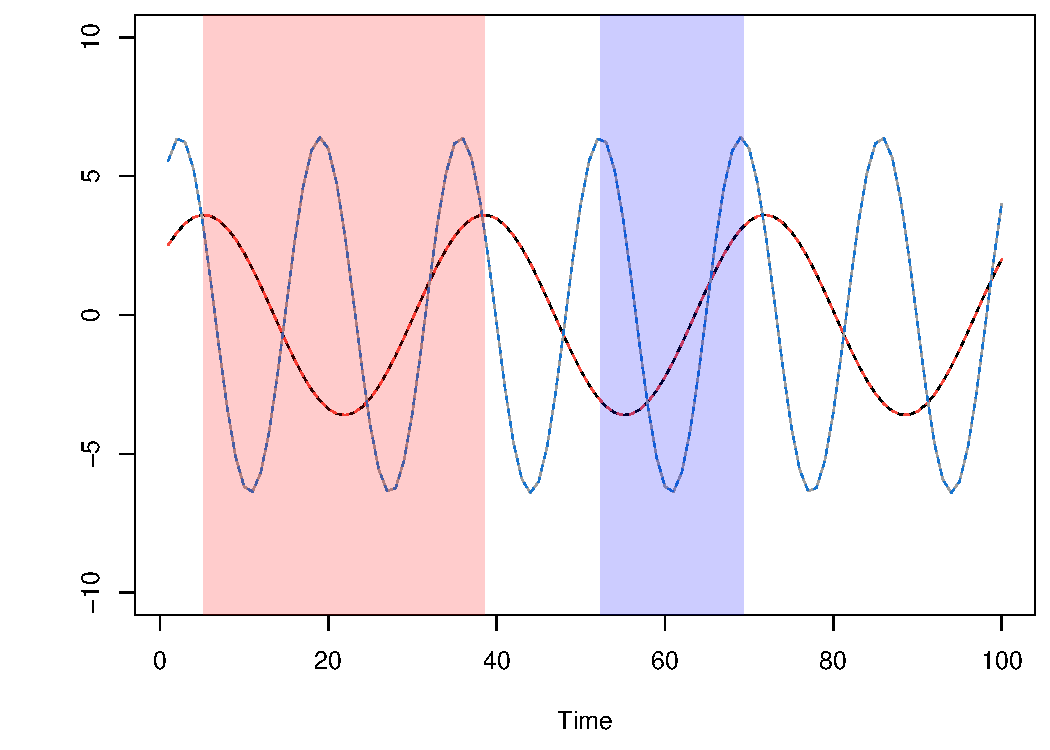
\includegraphics[width=0.875\textwidth]{fig/cos-process-1.pdf}
\caption{Two examples of cosine processes, the first (in red) having a frequency  
  $\omega = 3/100$ and amplitude \smash{$\sqrt{2^2 + 3^2} \approx 3.6$}, and the
  second (in blue) having a frequency $\omega = 6/100$ and amplitude
  \smash{$\sqrt{4^2 + 5^2} \approx 6.4$}.} 
\label{fig:cos-process}
\end{figure}

\item The quantity $A$ is called the \emph{amplitude} and $\phi$ the
  \emph{phase} of the process. The amplitude controls how high the peaks are, 
  and the phase determine where (along the cosine cycle) the process starts at
  the origin $t=0$   

\item We can introduce randomness into the process \eqref{eq:cos-process} by
  allowing $A$ and $\phi$ to be random

\item It will be useful to reparametrize. In general, recall the trigonometric
  identity (cosine compound angle formula):
  \begin{equation}
  \label{eq:compound-angle}
  \cos(a + b) = \cos(a) \cos(b) - \sin(a) \sin(b)
  \end{equation}
  Thus, starting with \eqref{eq:cos-process}, we can rewrite this as $x_t$ = $A
  \cos(\phi) \cos(2\pi\omega t) - A \sin(\phi) \sin(2\pi\omega t)$. Simply
  letting $U_1 = A \cos(\phi)$, $U_2 = -A \sin(\phi)$, we can therefore write   
  \begin{equation}
  \label{eq:cos-sin-process}
  x_t = U_1 \cos(2\pi\omega t) + U_2 \sin(2\pi\omega t)
  \end{equation}
  with $U_1, U_2$ our two random variables, determining the amplitude of the
  cosine and sine components separately

\item Note that another way of writing the relationship between $A,\phi$ and
  $U_1,U_2$ is (why?):
  \[
  A = \sqrt{U_1^2 + U_2^2}, \quad \phi = \tan^{-1}(-U_2/U_1)
  \]

  \item An interesting fact (that you can try to verify as a challenge): 
  \[
  U_1,U_2 \sim N(0,1), \text{ independently} \iff 
  A \sim \chi^2_2, \; \phi \sim \mathrm{Unif}(-\pi,\pi), \text{ independently} 
  \]
\end{itemize}

\subsection{Stationarity}

\begin{itemize}
\item If $U_1,U_2$ are uncorrelated, each with mean zero and variance
  $\sigma^2$, then the periodic process $x_t$, $t = 0, \pm 1, \pm 2, \dots$
  defined in \eqref{eq:cos-sin-process} is stationary

\item To check this: simply compute the mean function
  \[
  \mu_t = \E(x_t) = 0
  \]
  which is constant in time; and the autocovariance function 
  \begin{align*}
  \gamma(s,t) &= \Cov(x_s, x_t) \\
  &= \Cov\Big( U_1 \cos(2\pi\omega s) + U_2 \sin(2\pi\omega s), \, 
    U_1 \cos(2\pi\omega t) + U_2 \sin(2\pi\omega t) \Big) \\
  &= \Cov\Big( U_1 \cos(2\pi\omega s), \, U_1 \cos(2\pi\omega t) \Big) +
    \Cov\Big( U_2 \sin(2\pi\omega s), \, U_1 \cos(2\pi\omega t) \Big) \\
  &\qquad + \Cov\Big( U_1 \cos(2\pi\omega s), \, U_2 \sin(2\pi\omega t) \Big) +  
     \Cov\Big( U_2 \sin(2\pi\omega s), \, U_2 \sin(2\pi\omega t) \Big) \\
  &=\sigma^2 \cos(2\pi\omega s) \cos(2\pi\omega t) + 0 + 0 + \sigma^2
    \sin(2\pi\omega s) \sin(2\pi\omega t) \\
  &= \sigma^2 \cos(2\pi\omega (s-t))
  \end{align*}
  which only depends on the lag $s-t$ (where in the last line we used the
  identity \eqref{eq:compound-angle} once again)
\end{itemize}

\subsection{General mixtures}

\begin{itemize}
\item As a generalization of \eqref{eq:cos-sin-process}, we can also mix
  together a total of $p$ periodic processes, defining
  \begin{equation}
  \label{eq:cos-sin-process-p}
  x_t = \sum_{i=1}^p \Big( U_{k1} \cos(2\pi\omega_k t) + U_{k2}
  \sin(2\pi\omega_k t) \Big) 
  \end{equation}
  for $U_{k1}, U_{k2}$, $k = 1,\dots,p$ all uncorrelated random variables with
  mean zero, where $U_{k1}, U_{k2}$ have variance $\sigma^2_k$

\item As a generalization of the above calculation, you'll show on your homework
  that the process $x_t$, $t = 0, \pm 1, \pm 2, \dots$ defined in
  \eqref{eq:cos-sin-process-p} is stationary, with autocovariance function 
  \[
  \gamma(h) = \sum_{k=1}^p \sigma^2_k \cos(2\pi\omega_k h)
  \]

\item Figure \ref{fig:cos-mixture} displays a couple of mixture processes of the 
  form \eqref{eq:cos-sin-process-p} (with $p=2$ and $p=3$). Note the regular
  repeating nature of the mixture processes. One might wonder how we can
  decompose a such a mixture into its frequency components (periodic processes,
  each of the form \eqref{eq:cos-sin-process}). This is, in fact, one of the
  main objectives in spectral analysis

\begin{figure}[htb]
\centering
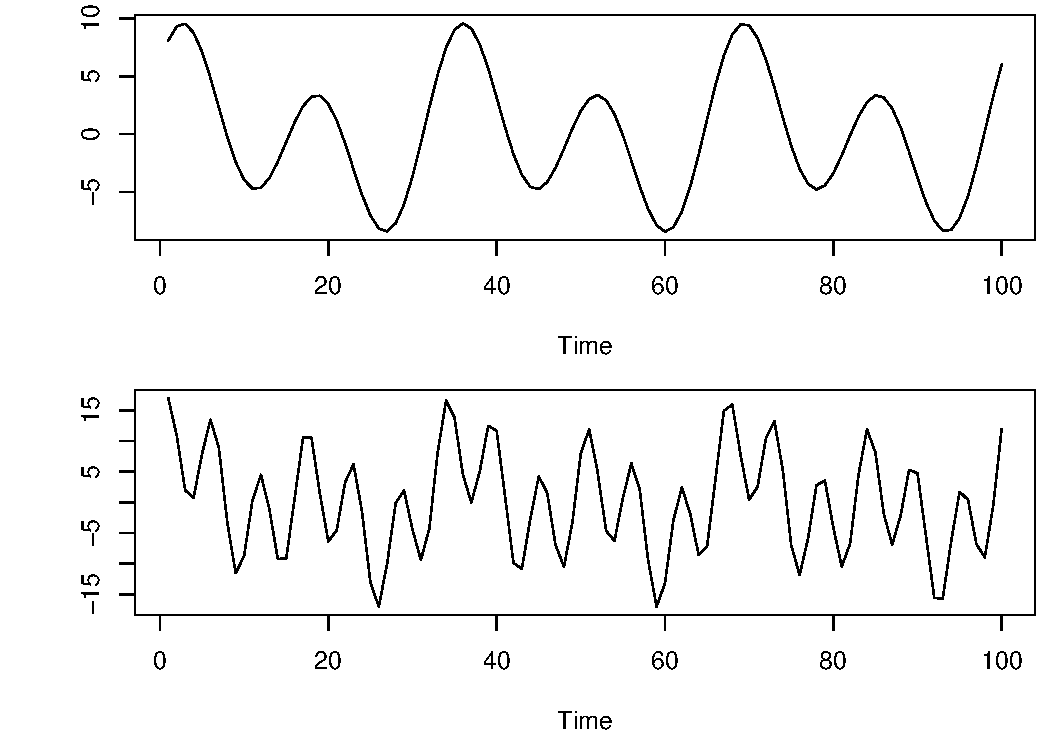
\includegraphics[width=0.875\textwidth]{fig/cos-mixture-1.pdf}
\caption{Mixture of periodic processes of different frequencies (and
  amplitudes).}  
\label{fig:cos-mixture}
\end{figure}

\item And the answer, as we'll see next, is given by something you're already
  quite familiar with ... regression! 
\end{itemize}

\section{Periodogram}

\section{Spectral density}

\section{Linear filtering}

\section{Lagged regression}

\end{document}
